En este ejemplo, los datos disponibles presentan un comportamiento estacional, 
evidenciado por los picos máximos y mínimos que se repiten periódicamente a lo 
largo del tiempo, como se muestra en la \cref{fig:graphic1}. Para predecir la 
demanda del primer trimestre del año siguiente (correspondiente a los valores 
16, 17, 18, 19 y 20), es necesario desestacionalizar los datos. Para ello, se 
utilizó el método de promedios móviles.

\begin{figure}[H]
    \centering
    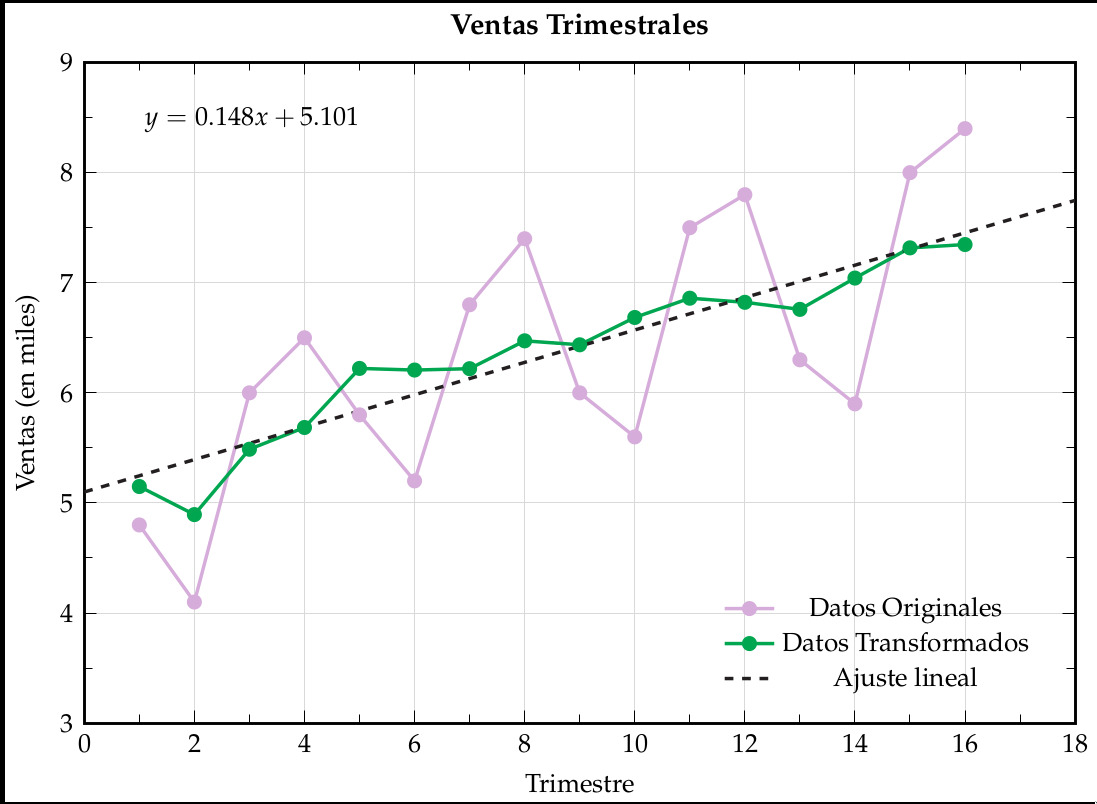
\includegraphics[width=0.5\linewidth]{images/graphic1.png}
    \label{fig:graphic1}
\end{figure}

Este método consiste en calcular el promedio de cuatro valores consecutivos de 
demanda, comenzando con los correspondientes a los trimestres 1, 2, 3 y 4, 
luego con los trimestres 2, 3, 4 y 5, y así sucesivamente hasta llegar al 
promedio de los trimestres 13, 14, 15 y 16. Cada uno de estos promedios se 
ubica en la posición intermedia entre el segundo y el tercer valor del grupo 
correspondiente. Sin embargo, dado que esa ubicación no coincide con ningún 
trimestre específico, es necesario calcular un nuevo promedio entre cada par de 
promedios consecutivos ya obtenidos. El resultado de este segundo promedio se 
asigna a la fila situada entre ambos valores originales. Estos nuevos valores 
corresponden a la columna denominada \textit{Promedio centrado} en la 
\cref{tab:table}.

A continuación, se divide cada valor de demanda entre su respectivo promedio 
centrado, obteniendo así un coeficiente por cada trimestre de demanda. Por 
ejemplo, el coeficiente de 1.1 corresponde al trimestre de demanda 3, mientras 
que el valor 0.97 se asocia al trimestre de demanda 1, y no al 5, debido a que 
cada trimestre del año agrupa cuatro valores de demanda. Una vez realizados 
estos cálculos, se agrupan los coeficientes según el trimestre al que 
pertenecen y se calcula el promedio de cada grupo. De esta manera, se obtienen 
los coeficientes de desestacionalización, que son únicamente cuatro.

Para obtener los valores de demanda desestacionalizada, se debe dividir cada 
valor de demanda entre su coeficiente de desestacionalización correspondiente 
(ya sea del primer, segundo, tercer o cuarto trimestre). Una vez 
desestacionalizados, los datos muestran un comportamiento lineal, como se 
observa en la \cref{fig:graphic1}. Por lo tanto, se procede a realizar un ajuste 
lineal, del cual se obtiene la siguiente ecuación:

\begin{equation}
    y = 0.148x + 5.101
    \label{eq:equation1}
\end{equation}

Con la \cref{eq:equation1}, se calculan los valores de demanda 
desestacionalizada para los trimestres 17, 18, 19 y 20, sustituyendo en la 
ecuación el valor de $x$ por cada uno de estos trimestres. A los resultados 
obtenidos se les añade el margen de error, el cual se calcula mediante la 
siguiente ecuación:

\begin{equation*}
    mr = \sqrt{\frac{\sum y^2 - a(\sum y - b\sum xy)}{n-2}}
\end{equation*}

En donde:
\begin{itemize}
    \item La variable $y$ corresponde a los valores de demanda desestacionalizada.
    \item $n = 16$
    \item $a = 0.148$
    \item $b = 5.101$
\end{itemize}

Una vez obtenidos los valores de demanda desestacionalizada para el primer 
trimestre del año siguiente, cada uno debe multiplicarse por su coeficiente de 
desestacionalización correspondiente. De este modo, se obtienen los valores de 
demanda real para dichos trimestres. En la \cref{fig:graphic2} se muestra la 
gráfica con los valores de demanda correspondientes a los cinco trimestres 
presentados en la \cref{tab:table}.
 
\begin{figure}[H]
    \centering
    \includegraphics[width=0.5\linewidth]{images/graphic2.png}
    \label{fig:graphic2}
\end{figure}

\begin{table*}[]
\pgfplotstabletypeset[
    col sep=comma,
    columns/Month/.style = {string type},
]{table.csv}
\label{tab:table}
\end{table*}
